\documentclass[10pt]{article}
\usepackage[english]{babel}
\usepackage[utf8]{inputenc}
\usepackage{a4}
\usepackage{amsmath}
\usepackage[pdftex]{graphicx}
\usepackage{verbatim}
\usepackage{url}
\usepackage{listings}
\usepackage{xcolor}
\topmargin -0.5in \textheight 9.0in \oddsidemargin 0.0in
\evensidemargin 0.0in \textwidth 6.5in
\graphicspath{{images/}}

\usepackage{titling}
\predate{}
\postdate{}

\definecolor{codegreen}{rgb}{0,0.6,0}
\definecolor{codegray}{rgb}{0.5,0.5,0.5}
\definecolor{codepurple}{rgb}{0.58,0,0.82}
\definecolor{backcolour}{rgb}{0.95,0.95,0.92}

\lstdefinestyle{mystyle}{
    backgroundcolor=\color{backcolour},   
    commentstyle=\color{codegreen},
    keywordstyle=\color{magenta},
    numberstyle=\tiny\color{codegray},
    stringstyle=\color{codepurple},
    basicstyle=\ttfamily\footnotesize,
    breakatwhitespace=false,         
    breaklines=true,                 
    captionpos=b,                    
    keepspaces=true,                 
    numbers=left,                    
    numbersep=5pt,                  
    showspaces=false,                
    showstringspaces=false,
    showtabs=false,                  
    tabsize=2
}
\lstset{style=mystyle}

\begin{document}

\title{Computer Vision Report: Lab 1}
\author{John Doe \& Jane Smith}
\date{}
\maketitle

\subsection*{Question 1}
\textbf{Why did the chicken cross the road?}\\
To get to the other side.

\subsection*{Exercise 1}

\begin{figure}[h]
\begin{center}
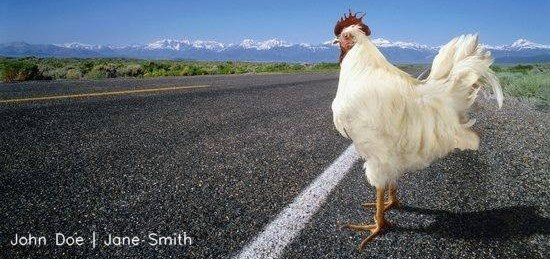
\includegraphics[width=0.75\textwidth]{chicken_named.jpg}
\end{center}
\end{figure}

\subsection*{Code}
\begin{lstlisting}[language=Python]
import cv2

def print_name(im, name):
	im = cv2.putText(im, name, (10, im.shape[0]-15), cv2.FONT_HERSHEY_SIMPLEX, 0.5, (255,255,255), 1, cv2.LINE_AA)
	return im

chicken = cv2.imread("chicken.jpg")
chicken = print_name(chicken, "John Doe | Jane Smith")
cv2.imwrite("chicken_named.jpg", chicken)

cv2.namedWindow("chicken")
cv2.imshow("chicken", chicken)
cv2.waitKey()
cv2.destroyAllWindows()
\end{lstlisting}

\end{document}
